\documentclass[a4paper, 12pt]{book} % changed from scrbook
% not using \documentclass[a4paper, twoside=semi]{scrreprt} anymore

\usepackage{InfoSec}

\definecolor{bg}{RGB}{20,20,20}
\definecolor{fg}{RGB}{220,220,220}
\definecolor{keyword}{RGB}{130,170,255}
\definecolor{comment}{RGB}{120,120,120}
\definecolor{string}{RGB}{255,200,120}

\lstdefinestyle{darkbash}{
    backgroundcolor=\color{bg},
    basicstyle=\scriptsize\ttfamily\color{fg},
    keywordstyle=\color{keyword},
    commentstyle=\color{comment},
    autogobble=true,
    stringstyle=\color{string},
    breaklines=true,
    showstringspaces=false,
    frame=single
}

% \usepackage{titlesec}
% \setkomafont{chapter}{\Huge\bfseries}
% \setkomafont{section}{\Large\bfseries}
% \setkomafont{subsection}{\large\bfseries}
\usepackage{fancyhdr, lastpage}
\usepackage{lstautogobble}
\usepackage{euscript}


\makeatletter
\providecommand{\subtitle}[1]{\gdef\@subtitle{#1}}
\providecommand{\@subtitle}{}
\makeatother


\usepackage{booktabs}
\usepackage{array}
\usepackage{multirow}




\usepackage{newfloat}
%\usepackage{tocloft}

% % Define new float environment
% \DeclareFloatingEnvironment[
%   fileext=lof,
%   listname={List of Flowcharts},
%   name=Flowchart,
% ]{flowchart}


\pagestyle{fancy}
%\fancyhf{}
\lhead{}
\chead{}
%\rhead{Introduction to the Theory of Computation}
\cfoot{\thepage\ of \pageref{LastPage}}
\rfoot{Version 8.3}




\RequirePackage{etex} 


%--- The documentation for the title can be found at: https://en.wikibooks.org/wiki/LaTeX/Title_Creation
\title{Information Security}
\author{Ahmed U. Ashraf}
\date{\today }
% \subtitle{Version~\version}

\begin{document}

% \include{glossary}


\maketitle
%--- we would like to hyperlink each item in contensts page
% \let\hypercontentsline=\contentsline
% \renewcommand{\contentsline}[4]{\hypertarget{toc.#4}{}\hypercontentsline{#1}{#2}{#3}{#4}}
%--- We print ToC: Table of Contents

\DeclareFontShape{U}{stmry}{b}{n}{<-> ssub * stmry/m/n}{}

\tableofcontents\label{toc}
%--- We print the list of figures, this might go at the end.




% \listoffigures
% %--- We print the list of tables, this might also go at the end.
% \listoftables
% %--- This is to add list of symbols as glossary
% % \printunsrtglossary[type=symbols,style=long,title={List of Symbols}]


% % List of Algorithms (- taken the idea from Discrete Algorithmic Mathematics by Stephen B.Maurer and ANthony Ralston.pdf)

% \listofalgorithms
% \addcontentsline{toc}{chapter}{List of Algorithms}

% \listofflowcharts
% %\addcontentsline{toc}{chapter}{List of Flowcharts}


\newpage


\chapter*{Foreword}
\begin{epigraph}
{Continuous improvement is better than delayed perfection.}{Mark Twain}
\end{epigraph}

\chapter{Computer Security}



Here are security properties of interest:
\begin{enumerate}
    \item \emph{Confidentiality}: the individual assets are only accessible to authorised parties.
    \item \emph{Integrity}: the individual assets can only be modified by authorised parties in authorised ways.
    \item Authorization:
    \item \emph{Availability}: the authorised parties can access the assets to an agreed extent. 
    \item Authentication:
    \item Accountability:
\end{enumerate}


\section{Design principles}

Here are design principles for computer security:
\begin{enumerate}
    \item Simplicity and necessity:
    \item Safe defaults:
    \item Open design:
    \item Complete mediation:
    \item Isolated compartments:
    \item Least privilege:
    \item Modular design:
    \item Small trusted bases:
    \item Time-tested tools:
    \item Least surprise:
    \item 
\end{enumerate}


\section{Risk Management}

The following are risk-mitigating strategies:
\begin{enumerate}
    \item \emph{Risk avoidance}: Keep the target system away from given risks.
    \item \emph{Risk reduction}: Take proactive steps to prevent losses occurring or to reduce the extent of the loss.
    \item \emph{Risk retention}: Allow a certain, agreed amount of ``residual risk''.
    \item \emph{Risk transfer}: Transfer the risk to others.
    \item \emph{Risk sharing}: Agree with other parties to deal with risks jointly.
\end{enumerate}


\chapter{Network Layers}
Here are the two models: OSI ISO model is abstraction-based, while TCP/IP model is implementation based.
\begin{longtable}{|c|c|c|} \hline 
    
    No. & Name & Job \\ \hline 
   7 & Application & Provide network process to application \\ \hline 
   6 & Presentation & Format conversion, encryption/decryption \\ \hline 
   5 & Session & Interhost communication, logon/off \\ \hline 
   4 &  Transport & Reliability, error check, flow control \\ \hline 
   3 &  Network & Logical addressing, routing \\ \hline 
   2 & Data Link & Physical addressing, link error check \\ \hline 
   1 &  Physical & Electrical signaling, cabling \\ \hline   
   \caption{\emph{Open Systems Interconnection} (OSI)  \emph{International Organization for Standardization} (ISO) model}      
\end{longtable}

\begin{longtable}{|c|c|c|} \hline 
    No. & Layer & Protocols \\ \hline 
    7 & Application & FTP, HTTP, SMTP, DNS \\ \hline 
    4 & Transport & TCP, UDP \\ \hline 
    3 & Internet & IP \\ \hline 
    1 & Network Access & Ethernet, MAC \\ \hline 
    \caption{TCP/IP model}
\end{longtable}

Message moves down through layers on sending device. When data reaches physical layer, it is changed into electromagnetic signal and sent along a physical link. Message then moves up through layers at the receiving device. Note that at intermediate nodes (routers), data is pulled only up to network layer, so that next hop could be determined.

Each layer encapsulates data sent by the layers above it and provides specific features to higherlayer protocols.

\begin{figure}[H]
    \centering
    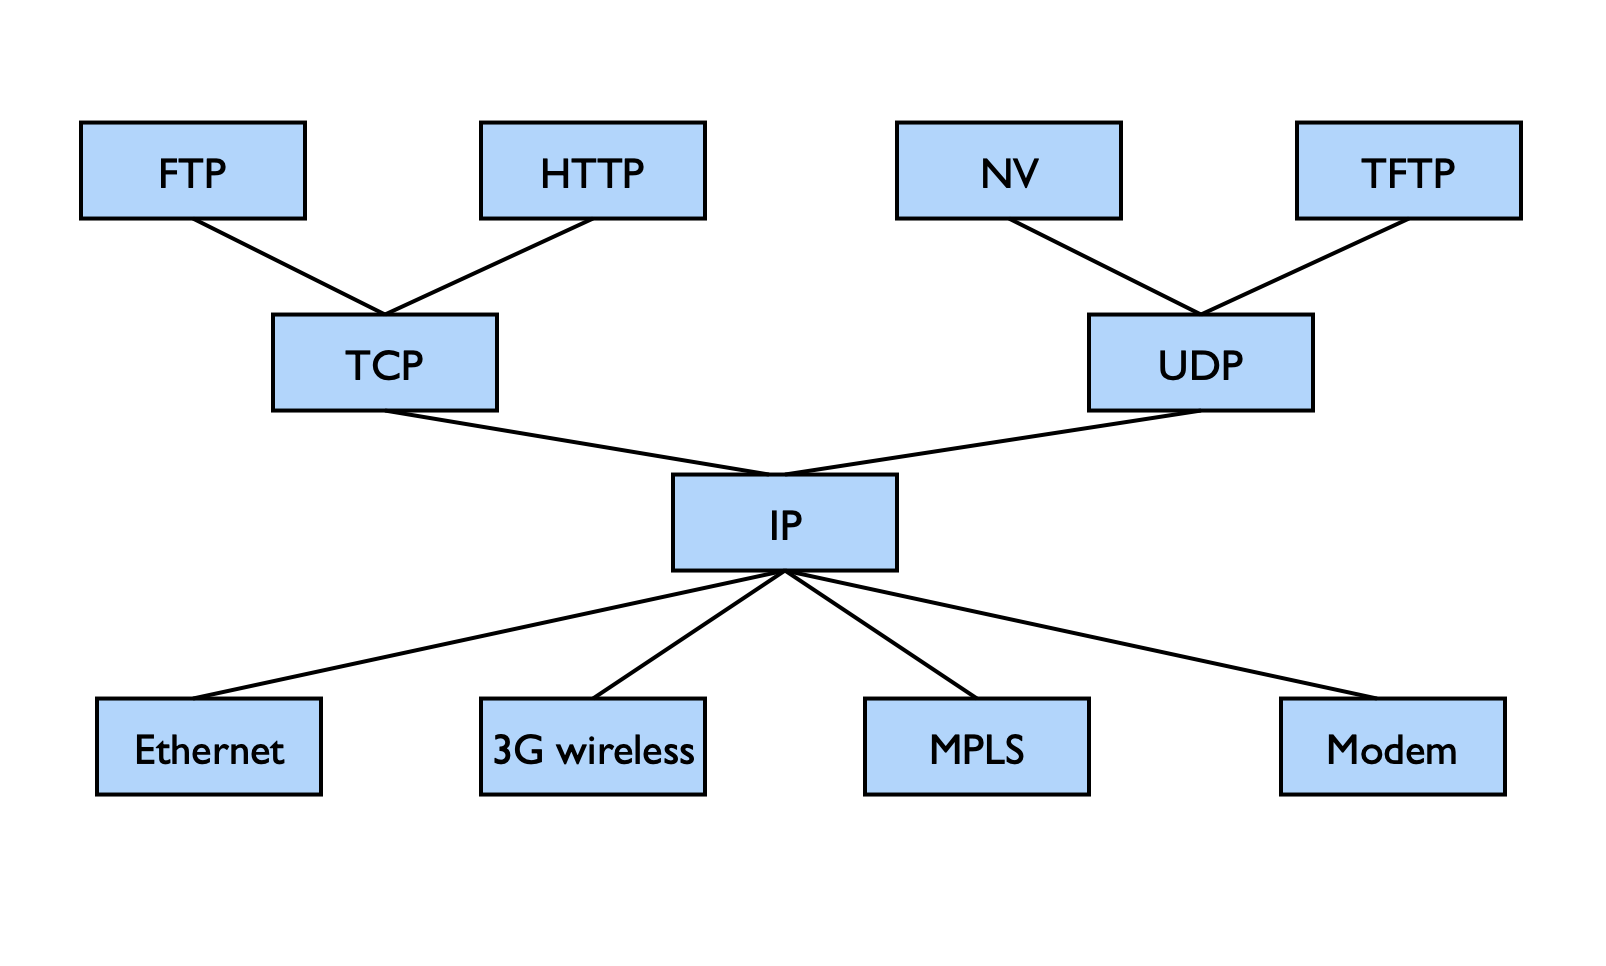
\includegraphics[scale=0.3]{hourglass.png}
    \caption{Internet Hourglass architecture}
\end{figure}






\section{IP}

We can check our configurations using the command for \emph{interface configuration}
\begin{lstlisting}[style=darkbash, language=bash]
ifconfig
\end{lstlisting}
This shows local IP. To check public IP, we use \textcolor{blue}{curl}
\begin{lstlisting}[style=darkbash, language=bash]
curl ifconfig.me
\end{lstlisting}
To find IP of others, we can use \textcolor{blue}{dig} or \textcolor{blue}{nslookup}
\begin{lstlisting}[style=darkbash, language=bash]
dig google.com
nslookup google.com
\end{lstlisting}
Given an public IP address, we can also ask who is at that address by using \textcolor{blue}{whois}
\begin{lstlisting}[style=darkbash, language=bash]
whois 192.178.192.138
\end{lstlisting}




\chapter{Probability}

A \emph{measurable space} $(\Omega, \EuScript{S})$ is a pair consisting of a \emph{sample space} $\Omega$ together with a $\sigma$-algebra $\EuScript{S}$ called the \emph{event space}. A \emph{probability space} $(\Omega, \EuScript{S}, \mu)$ is a triple consisting of a sample space $\Omega$, a $\sigma$-algebra $\EuScript{S}$ and a probability measure $\mu: \EuScript{S} \longrightarrow \mathbb{R}$ that satisfies:
\begin{enumerate}
    \item \emph{Non-negativity}: $\mu(x) \geq 0$, for all $x \in \EuScript{S}$.
    \item \emph{Normalization}: $\mu(\Omega) = 1$.
    \item \emph{Countable additivity}: Given disjoint sets $x_i \in \EuScript{S}$, we have 
    \begin{align}
        \mu\bigg( \bigcup_{i=0}^\infty x_i \bigg) = \sum_{i=0}^\infty \mu(x_i)
    \end{align}
\end{enumerate}

\chapter{Information Theory}
Information theory was founded by Claude Shannon in 1948 as a discipline to study the quantification, storage, and communication of information. In the past decades, it has played a critical role in modern communication as well as many other applications in engineering and computer science.  
% Mutual information and the Kullback-Leibler (KL) divergence 


\section{Information}
Let us consider the space of all messages to have a probability distribution. The probability distribution tell us how likely is it that we get a certain message. So we have some information about the occurrence of each message. Once we have receive a message, we gain some amount of information. For example, if probability of given message is 1, then we do not gain any new information after the occurrence of that message. The gain in the amount of information depends on its probability of its occurrence. Therefore, we can write the amount of information conveyed by a message $x$ as $I(p_x)$. This is also referred to as \emph{suprisal}, as it measures the amount of surprise we have after observing the message. \emph{Desidarata}: We would like the function $I: [0,1] \longrightarrow \mathbb{R}_{\geq 0}$ to satisfy the following properties:
\begin{enumerate}
    \item \emph{Non-negativity}: The information conveyed by a message cannot be negative. It has to be at least 0, that is
    \begin{align}
        I(p_x) \geq 0
    \end{align}
    % \item If the event is definite, that is, if the probability of the occurrence of the event is 1, then the corresponding information conveyed by the event will be 0. That is, 
    % \begin{align}
    %     I(1) &= 0
    % \end{align}
    \item \emph{Additivity}: The information conveyed by composite independent messages is simply given by the sum of the individual information content. That is,
    \begin{align}
        I(p_x p_y) &= I(p_x) + I(p_y)
    \end{align}
    \item \emph{Continuity}: The information $I$ is a continuous function.
\end{enumerate}


% ref: Python for Probability, Statistics and Machine Learning by Jose Unpingco
The only mathematical operator that satisfies these relations is the logarithm operator (up tp scalar multiple). Therefore, we have the following definition:
\begin{definition}
    The \emph{Shannon} \emph{information content} (or \emph{uncertainty content}) of an outcome $X = x$ is defined by
    \begin{align}
    I(x) &\defn \log\left(  \frac{1}{\pr(X = x)} \right) \\
    &= -\log(p(x))
    \end{align}
\end{definition}
The unit of the information is bits, nats or Hartley (or decits), when the base of the logarithm is the number $2$, the Euler's number $e$, or the number 10, respectively. The Shannon information can be interpreted as quantifying the level of \emph{surprise} of a particular outcome.



\section{Entropy}
% ref: The Probabilistic Method by Noga Alon and Joel H.Spencer
% ref: Statistical Properties of Deterministic Systems by Jiu Ding and Aihui Zhou
% ref: Permutation Complexity in Dynamical Systems by Jose M.Amigo
% ref: Pattern recognition and machine learning by Christopher M.Bishop

Entropy is the amount of information provided by an observation of a random variable. It reflects the uncertainty associated with predicting the variable value. The larger the value of entropy, the greater the uncertainty in predicting the value of an observation. If $p_x = 1$ (the outcome is certain), then observing $x$ yields $-\log(1) = 0$ units of information. On the other hand, observing X = 0 in this case yields $-\log(0) = \infty$: total surprise at observing an impossible outcome.

\begin{definition}
    The (\emph{Shannon}) \emph{entropy}\index{entropy} or \emph{uncertainty} of a discrete random variable $X$ with a probability distribution function $\pr: \EuScript{S} \longrightarrow [0,1]$ is defined by
    \begin{align}
        H(X) &\defn \sum_{x \in \EuScript{S}} \pr(X = x) \log\left( \frac{1}{\pr(X = x)} \right)  \\
        &= \mathrm{E}[I(X)]
    \end{align}
    If we restrict to binary logarithm $\log_2(\square)$, we refer to $H(X)$ as \emph{binary} (\emph{Shannon}) entropy. When the base is not mentioned, we assume that it to be 2. So mostly we are dealing with the binary entropy. We can also think of entropy as the average information. Observe that $\log(x)$ is undefined if $x = 0$. Hence, entropy is sometimes defined to be the relevant sum over all the non-zero probabilities\footnote{Also referred as $\supp(X)$}. However, since
        \begin{align}
        \lim_{x \longrightarrow 0} x \log\left( \frac{1}{x} \right) = 0
    \end{align}
    there is no real difficulty with allowing $\pr(x) = 0$ for some $x$'s. 
\end{definition}
Let us look at the entropy of the various components of a cryptosystem. We
can think of the key as being a random variable $k$ that takes on values in $k$, and hence we can compute the entropy $H(k)$. Similarly, we can compute entropies $H(P)$ and $H(C)$ of random variables associated with the plaintext and ciphertext, respectively. 

\begin{example}
    Let $\EuScript{P} = \{0,1\}$ with 

\end{example}

\begin{example}
    If $X$ is binary with two possible values $x_1$ and $x_2$ such that
    \begin{align}
        \pr(X = x_1) &= p \\
        \pr(X = x_2) &= 1-p
    \end{align}
    then 
    \begin{align}
        H(X) = - p \log(p) - (1-p)\log(1-p)
    \end{align}
\end{example}


\begin{example}
    \emph{Entropy of English language}:
\end{example}


\begin{definition}
    A real-valued function $f$ is a concave function on an interval $I$ if
    \begin{align}
        \frac{f(x) + f(y)}{2} &\leq f \bigg( \frac{x+y}{2} \bigg)
    \end{align}
    for all $x, y \in I$. A function $f$ is a strictly concave function on an interval $I$ if
    \begin{align}
        \frac{f(x) + f(y)}{2} &< f \bigg( \frac{x+y}{2} \bigg)
    \end{align}
    for all $x, y \in I$, $x \neq y$.
\end{definition}

\begin{theorem}
    (\emph{Jensen's inequality}) Suppose $f$ is a continuous strictly concave function on the interval $I$. Suppose further that
    \begin{align}
        \sum_{i=1}^n a_i = 1
    \end{align}
    and $a_i > 0$, for $1 \leq i \leq n$. Then 
    \begin{align}
        \sum_{i=1}^n a_i f(x_i) &\leq f\bigg( \sum_{i=1}^n a_i x_i\bigg)
    \end{align}
    where $x_i \in I$, for $1 \leq i \leq n$. Further, equality occurs if and only if $x_1 = \ldots = x_n$.
\end{theorem}
% ref: Cryptography Theory and Practice by Douglas R.Stinson and Maura B.Paterson
We now proceed to derive several results on entropy

% There is also notion of entropy for (symbolic) dynamical systems for example logistic map.
Since entropy is a mathematical measure of uncertainty, it is natural to
expect that when $\pr(X =k) = \dfrac{1}{n}$, the corresponding value of $H$ is maximal.
\begin{proposition}
    Let $U_n$ denote the uniform distribution. 
    \begin{align}
        H(X) &\leq \log(n) 
    \end{align}
    for all $X$. The maximum is achieved if and only if $X \sim U_n$. In plain words, the maximum entropy is given if all the events occur equally often.
\end{proposition}
\begin{proof}
    
\end{proof}
% ref: An Introduction to Mathematical Cryptography by Jeffrey Hoffstein, Jill Pipher and Joseph H.Silverman
% ref: Basic Principles and Applications of Probability Theory by A.V.Skorokhod

\begin{proposition}
If a function $f: \EuScript{S}_n \longrightarrow [0, \infty]$ satisfy the requirements of continuity, weak additivity, monotonicity, branching and normalization, then
\begin{align}
    f(X) &= H(X)
\end{align}
\end{proposition}

Application of these include \emph{Huffman coding} and \emph{Error correcting codes}. Huffman codes are used in the JPEG and MPEG standards.
% ref: Cryptography and Data Security by Dorothy Elizabeth Robling Denning


\begin{definition}
    Let $X$ and $Y$ be two discrete random variables with the event space $\EuScript{S}$ and $\EuScript{T}$, respectively. The \emph{joint entropy} $H(X, Y)$ is defined as
    \begin{align}
        H(X, Y) &\defn \sum_{ \substack{x \in \EuScript{S} \\ y \in \EuScript{T}}} \pr(X = x, Y = y) \log\bigg( \frac{1}{\pr(X = x, Y = y)}\bigg) \\
        &= \sum_{ \substack{x \in \EuScript{S} \\ y \in \EuScript{T}}} p(x, y) \log \bigg( \frac{1}{p(x, y)}\bigg)
    \end{align}
    The \emph{conditional entropy} $H(X|Y)$ is defined as 
    \begin{align}
        H(X|Y) &\defn \sum_{y \in \EuScript{T}} p(y)H(X|Y=y) \\
        &= \sum_{\substack{x \in \EuScript{S} \\ y \in \EuScript{T}}} p(x, y) \log \bigg( \frac{1}{p(x|y)}\bigg)
    \end{align}
\end{definition}


% ref: Cryptography Theory and Practice by Douglas R.Stinson and Maura B.Paterson
\begin{theorem}
    Let $\mathscr{C} = (\EuScript{P}, \EuScript{C}, \EuScript{K}, \EuScript{E}, \EuScript{D})$ be a cryptosystem, then 
    \begin{align}
        H(K|C) = H(K) + H(P) - H(C)
    \end{align}
\end{theorem}

\section{Kullback-Leibler divergence}




\section{Perfect Secrecy}
A cryptosystem has perfect secrecy if the interception of a ciphertext gives
the cryptanalyst no information about the underlying plaintext and no in-
formation about any future encrypted messages.



% ref: Cryptography Theory and Practice by Douglas R.Stinson and Maura B.Paterson
\begin{definition}
    A cryptosystem has perfect secrecy if 
    \begin{align}
        \pr(x|y) = \pr(x)
    \end{align}
    for all $x \in \EuScript{P}$, $y \in \EuScript{C}$. That is, the \emph{a posteriori} probability that the plaintext is $x$, given that the ciphertext $y$ is observed, is identical to the \emph{a priori} probability that the plaintext is $x$.
\end{definition}








\chapter{Cryptographic  Fundamentals}

\emph{Cryptography} is the practice and study of techniques for secure communication in the presence of adverse third parties. \emph{Encryption} refers to the process of changing ordinary text (plaintext) into unintelligible text (ciphertext). \emph{Decryption} is the reverse.

% references: 
% 1. Introduction to Cryptography with Maple by Jose Luis Gomez Pardo
% 2. Introduction to Cybersecurity by Robin Sharp
% 3. Understanding Cryptography by Christof Paar, Jan Pelzl and Tim Guneysu
% 4. Introduction to Cryptography by Hans Delfs and Helmut Knebl
% 5. Introduction to Computer Networks and Cybersecurity by Chwan-Hwa Wu and J.David Irwin
% 6. Handbook of Financial Cryptography and Security by Biurton Rosenberg
% 7. Guide to Internet Cryptography by Jorg Schwenk
% 8. Guide to Computer Network Security by Joseph Migga Kizza
% 9. Encrypt, Sign, Attack by Olaf Manz
% 10. Cryptograpy Theory and Practice by Douglas R.Stinson
% 11. Discovering Cybersecurity by Seth James Nielson
% 12. CryptoSchool by Joachim von zur Gathen copy
% 13. Cryptology by Richard Klima and Neil Sigmon
% 14. Cryptography by Douglas R.Stinson and Maura B.Paterson
% 15. Cryptography and Network Security by William Stallings 
% 16. Cryptographic Protocol by Ling Dong and Kefei Chen
% 17. Cryptography and Network Security by Marcelo Sampaio de Alencar
% 18. Computer Security Fundamentals by Chuck Easttom
% 19. Computer Security and the Internet by Paul C.van Oorschot
% 20. Computer Security and Cryptography by Alan G.Konheim.pdf
% 21. CompTIA Security Certification Study Guide by Ahmed F.Sheikh
% 22. Classical and Modern Cryptography for Beginners by Rajkumar Banoth and Rekha Regar
% 23. A Classical Introduction to Cryptography by Serge Vaudenay




\section{Cryptosystems}

Let $\Sigma_1, \Sigma_2$ be alphabets \footnote{Plain and cipher alphabet.}, and let $\ell_1, \ell_2$ be positive integers. We are interested in functions of the form $f: \Sigma_1^{\ell_1} \longrightarrow \Sigma_2^{\ell_2}$

\begin{definition}
    A \emph{cryptosystem}\index{cryptosystem} or an \emph{encryption-decryption scheme}\index{encryption-decryption scheme} is a quintuple $\mathscr{C} = (\EuScript{P}, \EuScript{C}, \EuScript{K}, \EuScript{E}, \EuScript{D})$ where 
    \begin{enumerate}
        \item The collection $\EuScript{P} \subseteq \Sigma_1^{\ell_1}$ is the set of all possible \emph{plain texts}, called the \emph{plaintext space}. It consists of elementary strings that are to be encrypted as a basic unit.
        \item The collection $\EuScript{C}  \subseteq \Sigma_2^{\ell_2}$ is the set of all possible \emph{cipher texts}, called the \emph{ciphertext space}.
        \item The collection $\EuScript{K}$, called the \emph{key space}, is the set of all possible \emph{keys}. This may come along with a (\emph{keystream}) generator $g: \EuScript{K} \longrightarrow \Sigma^\infty$, where $\Sigma$ is the keystream alphabet.
        \item The collection $\EuScript{E} = (e_k: \EuScript{P} \rightarrow \EuScript{C})_{k \in \EuScript{K}}$\footnote{In case of haveing a keystream generator, the indexing set of encryption-decryption maps is the keystream space. So we sometime have abuse of notation where $\EuScript{K}$ means $\Sigma^{\infty}$.} is a finite set of \emph{encryption rules} $e_k$, that are functions given by polynomial-time algorithms.
        \item The collection $\EuScript{D} = (d_{k'}: \EuScript{C} \rightarrow \EuScript{P} )_{k' \in \EuScript{K}}$ is a finite set of \emph{decryption rules}, that are functions given by polynomial-time algorithms.
    \end{enumerate}
    such that for each \emph{encryption key} $k \in \EuScript{K}$, there exists a \emph{decryption key} $k' \in \EuScript{K}$, which satisfies
    \begin{align}
        d_{k'} \circ e_k \equiv 1_{\EuScript{P}}
    \end{align}
    That is, 
    \begin{align}
        d_{k'}(e_k(x)) = x
    \end{align}
    for all $x \in \EuScript{P}$.
\end{definition}


The plaintext and ciphertext messages are elements of $\EuScript{P}^*$ and $\EuScript{C}^*$, respectively. Given a plaintext message 
\begin{align}
    \mathbf{x} = x_1 x_2 \cdots x_{j}  \in \EuScript{P}^* \footnotemark 
\end{align}
and a cryptosystem $\mathscr{C}$, with encryption maps $e_k$, one can encrypt $\mathbf{x}$ with a key $k$ (as in \emph{Block cipher}\index{Block cipher}) by \footnotetext{These $x_i$ are in $\EuScript{P}$.}
\begin{align}
    \mathbf{y} = e_k(x_1) e_k(x_2) \cdots e_k(x_{j})
\end{align}
or with a key stream $k_1k_2\cdots $ (as in \emph{Stream cipher}\index{Stream cipher})  by
\begin{align}
    \mathbf{y} = e_{k_1}(x_1) e_{k_2}(x_2) \cdots e_{k_j}(x_j)
\end{align}

If the encryption key $k$ always equal to the decryption key $k'$ or if $k'$ is easily computed from $k$, then the cryptosystem is called \emph{symmetric}. If the encyrption and decryption keys $k, k'$ are not equal and computation of $k'$ is infeasible from $k$, then the cryptosystem is called \emph{assymetric}.







\section{Shift cipher}
\begin{definition}
    Let $G$ be an additive group (for example, $\mathbb{Z}$ or $\mathbb{Z}_n$). Let $\EuScript{P} = \EuScript{C} = G$ and $\EuScript{K}$ be a subset of $G$. Recall that $G$ acts on itself via translation (shift) and so does any subset, in particular $\EuScript{K}$, acts on $G$. We can define a \emph{shift cipher}, by setting:
    \begin{align}
        e_k(x) &\setn x + k 
    \end{align}
    and
    \begin{align}
        d_k(y) &\setn y - k 
    \end{align}
    That is $\bigg(G, G, G, (g \cdot)_{g \in G}, (g^{-1} \cdot)_{g \in G} \bigg)$\footnote{Here the group $G$ is written multiplicatively.} is called a \emph{shift cipher}.
\end{definition}


\begin{example}
    The usual English-alphabet shift cipher: Let $\EuScript{P} = \EuScript{C} = \EuScript{K} = \mathbb{Z}_{26}$. For $0 \leq k \leq 25$, define 
    \begin{align}
        e_k(x) &\setn x + k \pmod{26}
    \end{align}
    and 
    \begin{align}
        d_k(y) &\setn y - k \pmod{26} 
    \end{align}
    Consider the usual encoding $\{0,1,\ldots,25\} \equiv \{A, B, \ldots, Z\}$ and take $k = 3$, then this corresponds to the \textsf{Caeser} cipher \index{Caeser cipher}.
\end{example}

\begin{example}
    Consider the shift cipher for $k = 11$ on the plaintext message:
    \begin{align}
        \texttt{wewillmeetatmidnight}
    \end{align}
    We first use encoding to write it as
    \begin{align}
        \begin{array}{cccccccccc}
            22 & 4 & 22 & 8 & 11 & 11 & 12 & 4 & 4 & 19 \\
            0 & 19 & 12 & 8 & 3 & 13 & 8 & 6 & 7 & 19
        \end{array}
    \end{align}
    We apply the encryption
    \begin{align}
        \begin{array}{cccccccccc}
            7 & 15 & 7 & 19 & 22 & 22 & 23 & 15 & 15 & 4 \\
            11 & 4 & 23 & 19 & 14 & 24 & 19 & 17 & 18 & 4
        \end{array}
    \end{align}
    Converting back, we obtain
    \begin{align}
        \texttt{HPHTWWXPPELEXTOYTRSE}
    \end{align}

\end{example}





\section{Substitution cipher}

\begin{definition}
    If $\EuScript{P} = \EuScript{C}$ is a set, say $X$ and $\EuScript{K}$ $= \mathfrak{S}(X)$ that acts on $S$ via permutation, then we can define a \emph{substitution cipher}, by defining:
    \begin{align}
        e_\pi(x) &= \pi(x) 
    \end{align}
    and
    \begin{align}
        d_\pi(y) &= \pi^{-1}(x) 
    \end{align}
    That is $(X, X, \mathfrak{S}(X), g \cdot, g^{-1} \cdot)$\footnote{Here the group $G$ is written multiplicatively.} is called a \emph{shift cipher}.

\end{definition}






\begin{example}
    (\emph{English-alphabet}) \emph{Substitution Cipher}: Let $\EuScript{P} = \EuScript{C} = \mathbb{Z}_{26}$. Let $\EuScript{K}$ $= \mathfrak{S}_{26}$ consists of all possible permutations of $\{0,1,2,\ldots, 25\}$. For each permutation $\pi \in \EuScript{K}$, define
    \begin{align}
        e_\pi(x) = \pi(x)
    \end{align}
    and 
    \begin{align}
        d_\pi(y) &= \pi^{-1}(y)
    \end{align}
    where $\pi^{-1}$ is the inverse permutation to $\pi$. \textsf{Atbash cipher} is an example of a substitution cipher. 
\end{example}






\section{Affine cipher}

\begin{example}
    (\emph{English-alphabet}) \emph{Affine Cipher}: Let $\EuScript{P} = \EuScript{C} = \mathbb{Z}_{26}$, and let 
    \begin{align}
        \EuScript{K} &= \{(a, b) \in \mathbb{Z}_{26} \times \mathbb{Z}_{26}: \gcd(a, 26) = 1\}
    \end{align}
    For $k = (a, b) \in \EuScript{K}$, define 
    \begin{align}
        e_k(x) &= (ax + b) \pmod{26} 
    \end{align}
    and 
    \begin{align}
        d_k(y) &= a^{-1}(y - b) \pmod{26}
    \end{align}
    \textsf{ROT13} is an instance of an affine cipher.
\end{example}


\section{Hill cipher}
\begin{example}
        (\emph{English-alphabet}) \emph{Hill Cipher}: Let $m \geq 2$ be an integer and let $\EuScript{P} = \EuScript{C} = (\mathbb{Z}_{26})^m$, and let 
    % \begin{align}
    %     \EuScript{K} &= \mathrm{GL}_m(\mathbb{Z}_{26}) = \{m\times m~\text{invertible matrices over}~\mathbb{Z}_{26}\}
    % \end{align}
    For a key $A_k \in \EuScript{K}$, we define 
    \begin{align}
        e_k(x) &= A_k x
    \end{align}
    and 
    \begin{align}
        d_k(y) &= y A_k^{-1}
    \end{align}
    where all operations are performed over $\mathbb{Z}_{26}$.
\end{example}





\section{Permutation cipher}


A permutation cipher is a special case of a Hill cipher.
\begin{definition}
    Let $S$ be a set and let $\ell$ be a positive integer. Let $\EuScript{P} = \EuScript{C} = S^\ell$, and let $\EuScript{K}$ $= \mathfrak{S}_\ell$. For a key $\pi \in \mathfrak{S}_\ell$, we set
    \begin{align}
        e_{\pi}(x_1, x_2, \ldots, x_m) &\setn (x_{\pi_1}, x_{\pi_2}, \ldots, x_{\pi_m})
    \end{align}
    and
    \begin{align}
        d_{\pi}(y_1, y_2, \ldots, y_m) &\setn (y_{\pi^{-1}_1}, y_{\pi^{-1}_2}, \ldots, y_{\pi^{-1}_m})   
    \end{align}
\end{definition}




\section{Autokey cipher}


\section{Modes of Encryption}


\begin{enumerate}
    \item \emph{Electronic CodeBook}(ECB): is the simplest block cipher mode of operation. It divides plaintext into fixed -size blocks and encrypts each independently using the same key. Because identical plaintext blocks always produce identical ciphertext blocks, it fails to hide data patters and is generally insecure.
    \item \emph{Cipher Block Chaining}(CBC): xors the plaintext woth the prior ciphertext block. The first block must use an \emph{initialization vector}(IV) because there is no prior block.
    \item \emph{Cipher FeedBack mode} (CFB): 
    \item  \emph{Output FeedBack mode} (OFB).


\end{enumerate}





The following modes create a stream cipher from a block cipher. 
\begin{enumerate}
    \item CounTeR mode (CTR).
\end{enumerate}








\section{Terminology}
\emph{Cryptography} is the study of how to alter a message so that someone intercepting it cannot read it without the appropriate algorithm and key. Here are some terms associated with this that we would like to define before starting:
\begin{longtable}{|l|p{10cm}|} \hline 
    Cipher & A synonym for the algorithm used to transform plain text to cipher text. \\  \hline 
    Cipher text & The coded or encrypted message. If your encryption is sufficiently strong, your cipher text should be secure  \\ \hline 
    Cryptanalysis\footnote{Sometimes referred as \emph{code breaking}.} & the study of principles and methods of deciphering cipher text without knowing the key \\ \hline 
    Decipher (decrypt) & Decipher and decrypt are synonyms. Both terms mean to convert the cipher text to plain text. \\ \hline 
    Encipher (encrypt) &  Encipher and encrypt are synonyms. Both words mean to convert the plain text into cipher text. \\ \hline 
    Key & The information, usually some sort of number, used with the algorithm to encrypt or decrypt the message.  \\ \hline 
    Key space  & The total number of possible keys that could be used. \\ \hline 
    Plain text & The original message—the information you want to secure. \\ \hline 
\end{longtable}




















\section{Finite Field Arithmetic}


\section{Diffie-Hellman (DH) protocol}

Diffie-Hellman (DH) is a mathematical protocol\footnote{A protocol can also be thought as a special case of an algorithm.} that allows two parties to securely establish a shared secret over an insecure public network. Once generated, this shared secret is typically used as an encryption key for faster symmetric algorithms like AES to communicate privately.

DH is still in use today, but certain precautions have to be taken with respect to its building blocks. Authentication also needs to be implemented on top of DH to prevent man-in-the-middle threats.

The mathematical basis for this algorithm is Discrete Logarithm Problem (DLP).


\section{Rivest-Shamir-Adleman (RSA) protocol}

Rivest-Shamir-Adleman (RSA) is an asymmetric cryptographic algorithm used by modern computers that relies on factoring integers.



\section{Models of encryption}

\subsection{Symmetric encryption model}
\begin{figure}[H]
    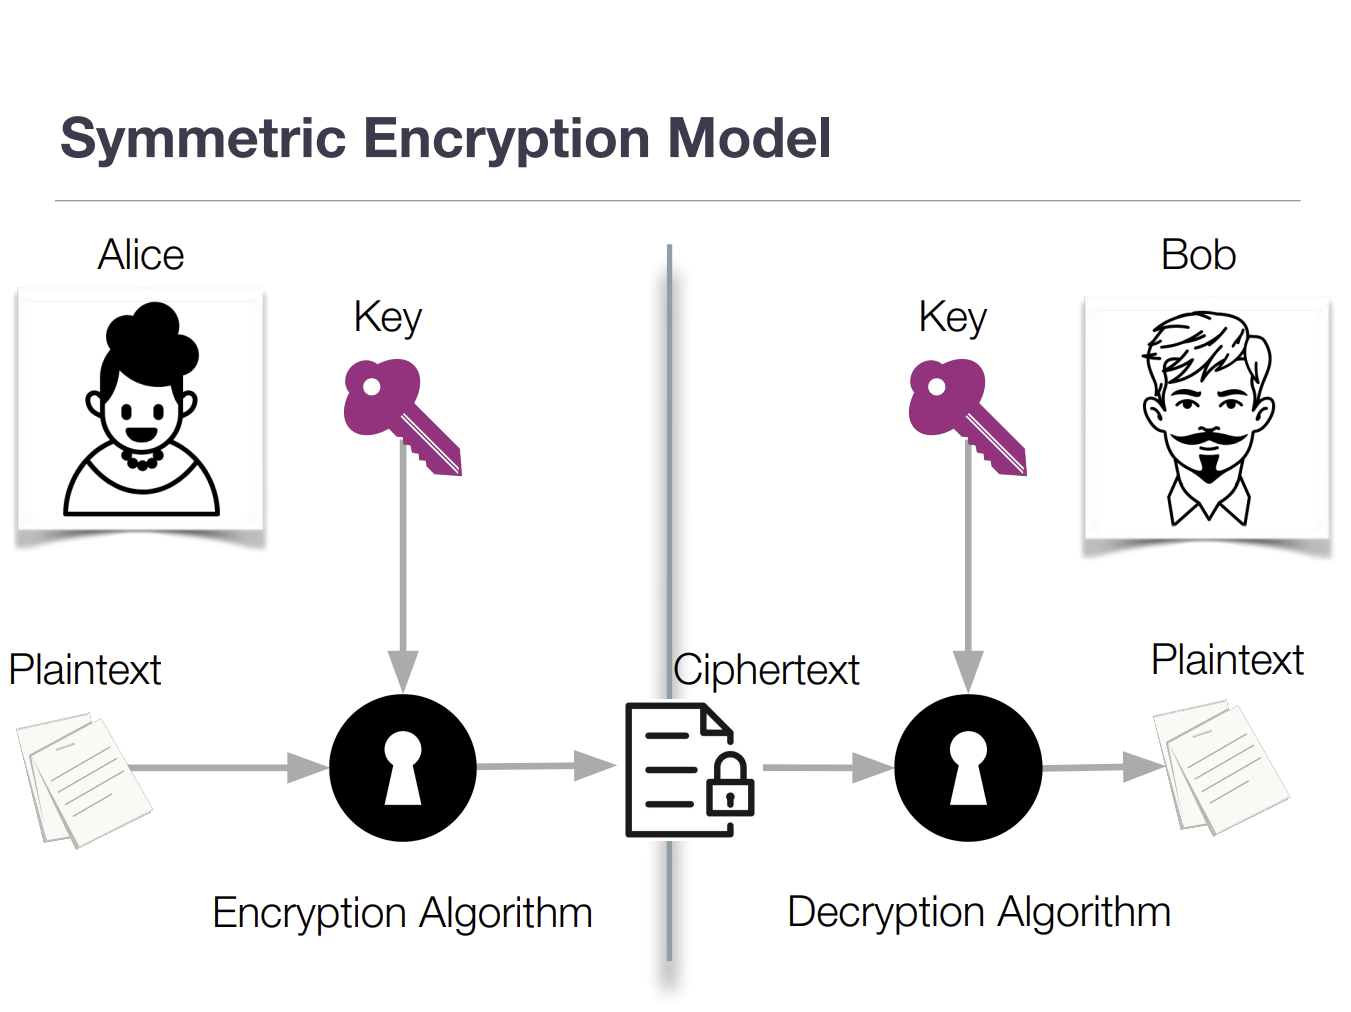
\includegraphics[scale=0.3]{symmetricmodel.png}
\end{figure}
The use cases for that are
\begin{enumerate}
    \item Web browsing using HTTPS.
    \item Encrypted chat (WhatsApp and Signal).
    \item Encrypted email (S/MIME and PGP).
    \item File and disk encryption.
\end{enumerate}

Requirements for symmetric encryption:
\begin{enumerate}
    \item Strong encryption.
    \item Fast.
    \item Sender and receiver must securely obtain and store secret key.
\end{enumerate}

\subsection{Public key encryption model}
\begin{figure}[H]
    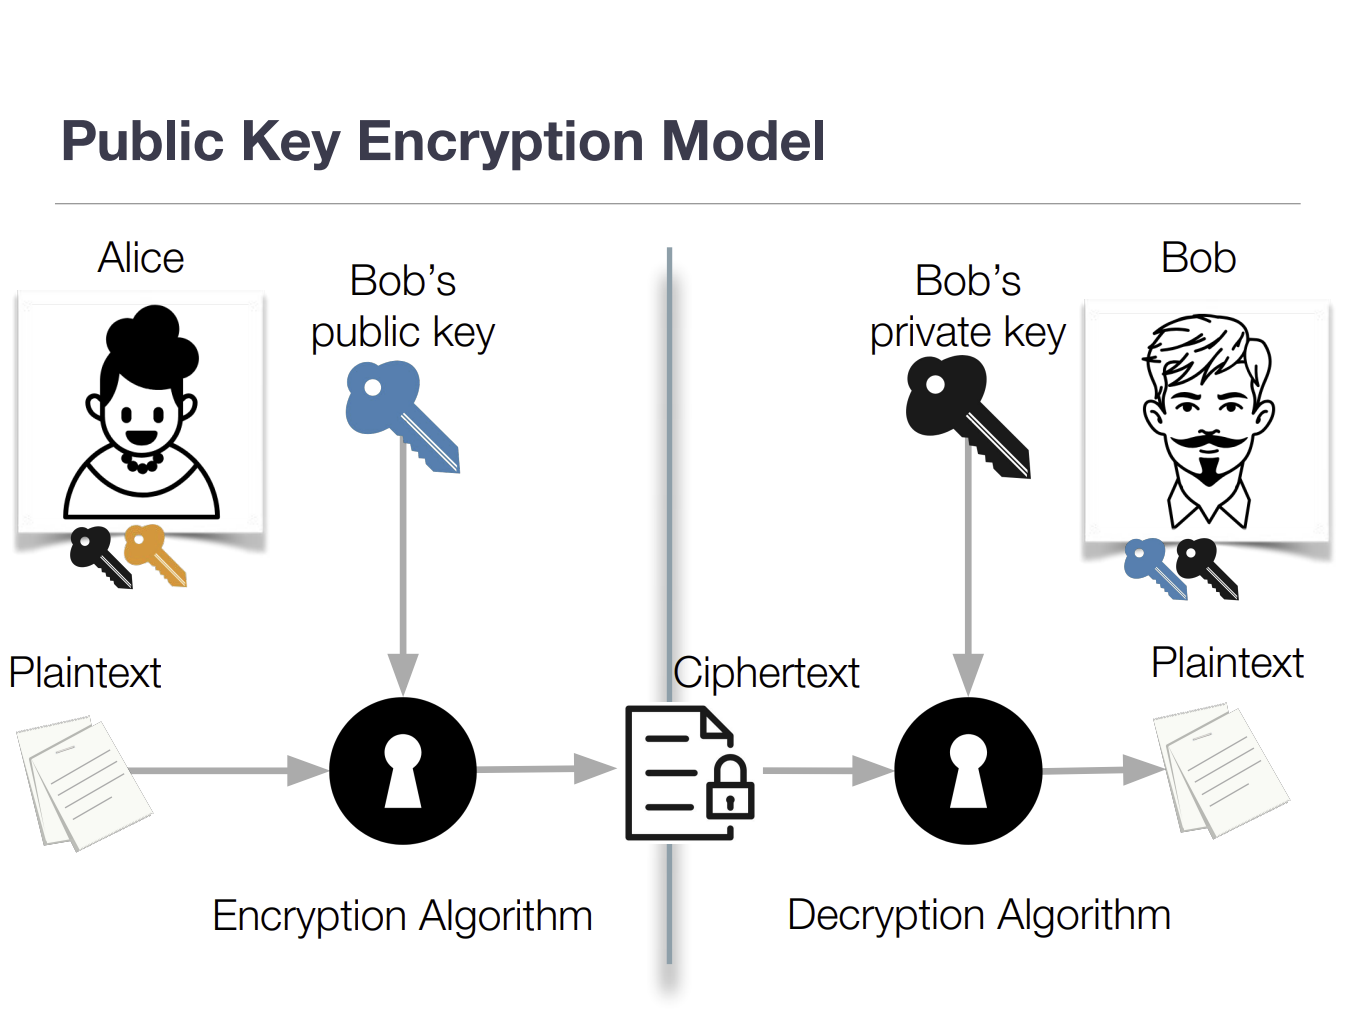
\includegraphics[scale=0.3]{publickey.png}
\end{figure}
The use cases for that
\begin{enumerate}
    \item Diffie-Hellman.
    \item RSA.
    \item Elliptic Curve Cryptography (ECC).
    \item Identity-based Encryption (IBE).
\end{enumerate}


\subsection{Public key digital signature model}
\begin{figure}[H]
    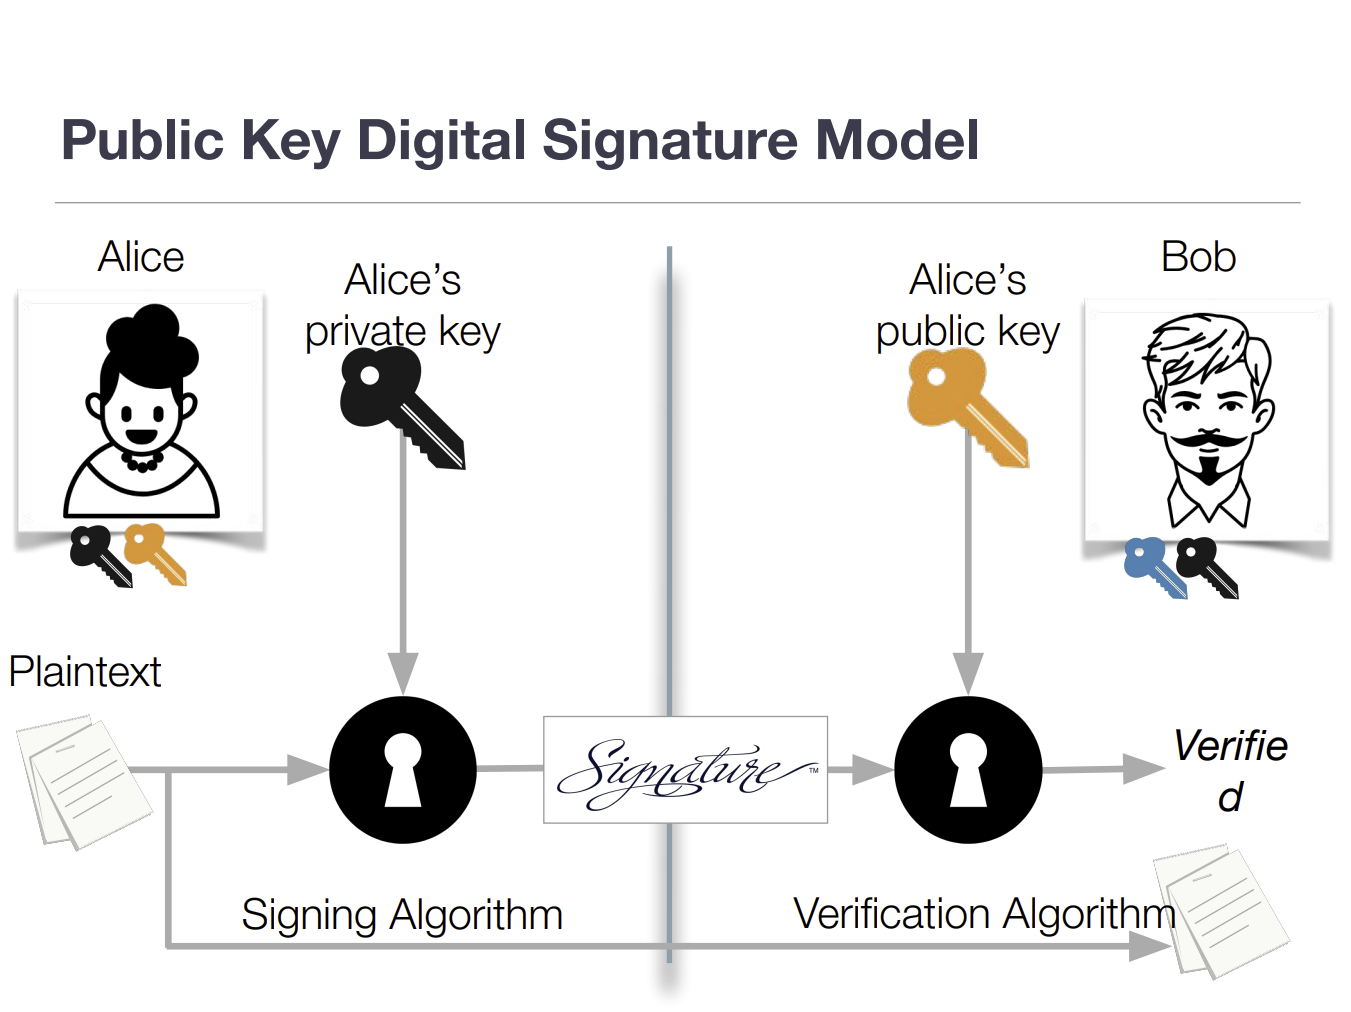
\includegraphics[scale=0.3]{publickeysign.png}
\end{figure}


\section{Cryptographic Hash Function}

These are one-way function\footnote{How can we make it rigorous.}. We desire the following properties from these functions, (call an arbitrary one $f$):
\begin{enumerate}
    \item It can be applied to a block of data of any size.
    \item It produces a fixed-length output.
    \item The value $f(x)$ is relatively easy to compute for any given $x$.
    \item \emph{One-way}: For any given value $h$, it is computationaly infeasible to find (any one of) its pre-image block $x$, that is such that $f(x) = h$.
    \item \emph{Weak collision resistant}: For any given block $x$, it is computationally infeasible to find $x' \neq x$ such that $f(x) = f(x')$.
    \item \emph{Strong collision resistant}: It is computationally infeasible to find any pair $(x, x')$ such that $f(x) = f(x')$.
\end{enumerate} 


Useful applications of hash function:
\begin{enumerate}
    \item Human-readable method to compare/verify data.
    \item Chaining events together - blockchain.
    \item Digital signatures and message authentication codes.
    \item Fundamental building block of many secure protocols.
\end{enumerate}

\begin{example}
    \emph{SHA-0}: Completely broken, collisions found.
    \emph{SHA-1}: Implemented using Merkle-Damg\.ard construction. 
    \emph{SHA-2}: No known flaws.
    \emph{SHA-3}: Subset of Keccak. Implemented using sponge construction.
\end{example}

\begin{example}
    \emph{MD5}: Completely broken, collisions found.
\end{example}




\chapter{Public Key Infrastructure (PKI)}

Public-key cryptography is a cryptographic technique that enables entities to securely communicate on an insecure public network, and reliably verify the identity of an entity via digital signatures. A \emph{public key infrastructure}\footnote{This includes Hardware, software and policies.} (PKI) is a system for the creation, storage, management, distribution and revokation of public keys and digital certificates, which are used to verify that a particular public key belongs to a certain entity. The PKI creates digital certificates that map public keys to entities, securely stores these certificates in a central repository and revokes them if needed. PKI consists of
\begin{enumerate}
    \item A \emph{certificate authority} (CA) which stores, issues, and signs digital certificates.
    \item A \emph{registration authority} (RA) which verifies the identity of entities requesting their digital certificates to be stored at the CA.
    \item A \emph{central directory}, a secure location in which keys are stored and indexed.
    \item A \emph{certificate management system}, which manages things like the access to stored certificates or the delivery of the certificates to be issued;
    \item A \emph{certificate policy}, which states the PKI's requirements concerning its procedures. Its purpose is to allow outsiders to analyze the PKI's trustworthiness.
\end{enumerate}


\section{Digital certificates}

Certificates are designed to bind a subject to the subject's public key. These certificates should be digitally signed by another entity called \emph{Certificate Authority} (CA).

\begin{example}
    OpenSSL, Let's Encrypt are examples of CA.
\end{example}


In order to get the certificate from the server \emph{google.com} of the host \emph{google.com}.
\begin{lstlisting}[style=darkbash, language=bash]
echo | \
openssl s_client \
-connect google.com:443 \
-servername google.com | \
openssl x509 \
-outform PEM \
> google_cert.pem
\end{lstlisting}


What does X.509 certificate contains:
\begin{table}[H]
    \begin{tabular}{|c|c|} \hline \\
        Version & $\texttt{3 (0x2)}$\\ \hline 
        Serial Number & $\texttt{\tiny 13:9c:df:29:a8:b5:bc:52:12:41:3e:ee:af:d1:8c:be}$ \\ \hline 
        Signature Algorithm & $\texttt{sha256WithRSAEncryption}$ \\ \hline 
        Issuer &  C=US, O=Google Trust Services, CN=WR2 \\
        Validity & \\
        Not Before & May 25 08:36:19 2026 \\
        Not After & Aug 17 08:36:18 2026 \\
        Subject & CN=*.google.com \\
        Subject Public Key Info &  \\
        Public Key Algorithm &  id-ecPublicKey \\
        NIST CURVE &  P-256 \\
        Public-Key & (256 bit) \\
    \end{tabular}
\end{table}

\section{Certificate Signing Requests (CSRs)}


\chapter{OpenSSL}



\section{Encodings}

\verb|openssl enc -list|


\begin{table}[H]
\centering
\small
\begin{tabular}{llll}
\hline
aes-128-cbc & aes-128-cfb & aes-128-cfb1 & aes-128-cfb8 \\
aes-128-ctr & aes-128-ecb & aes-128-ofb & aes-192-cbc \\
aes-192-cfb & aes-192-cfb1 & aes-192-cfb8 & aes-192-ctr \\
aes-192-ecb & aes-192-ofb & aes-256-cbc & aes-256-cfb \\
aes-256-cfb1 & aes-256-cfb8 & aes-256-ctr & aes-256-ecb \\
aes-256-ofb & aes128 & aes128-wrap & aes128-wrap-pad \\
aes192 & aes192-wrap & aes192-wrap-pad & aes256 \\
aes256-wrap & aes256-wrap-pad & aria-128-cbc & aria-128-cfb \\
aria-128-cfb1 & aria-128-cfb8 & aria-128-ctr & aria-128-ecb \\
aria-128-ofb & aria-192-cbc & aria-192-cfb & aria-192-cfb1 \\
aria-192-cfb8 & aria-192-ctr & aria-192-ecb & aria-192-ofb \\
aria-256-cbc & aria-256-cfb & aria-256-cfb1 & aria-256-cfb8 \\
aria-256-ctr & aria-256-ecb & aria-256-ofb & aria128 \\
aria192 & aria256 & bf & bf-cbc \\
bf-cfb & bf-ecb & bf-ofb & blowfish \\
camellia-128-cbc & camellia-128-cfb & camellia-128-cfb1 & camellia-128-cfb8 \\
camellia-128-ctr & camellia-128-ecb & camellia-128-ofb & camellia-192-cbc \\
camellia-192-cfb & camellia-192-cfb1 & camellia-192-cfb8 & camellia-192-ctr \\
camellia-192-ecb & camellia-192-ofb & camellia-256-cbc & camellia-256-cfb \\
camellia-256-cfb1 & camellia-256-cfb8 & camellia-256-ctr & camellia-256-ecb \\
camellia-256-ofb & camellia128 & camellia192 & camellia256 \\
cast & cast-cbc & cast5-cbc & cast5-cfb \\
cast5-ecb & cast5-ofb & chacha20 & des \\
des-cbc & des-cfb & des-cfb1 & des-cfb8 \\
des-ecb & des-ede & des-ede-cbc & des-ede-cfb \\
des-ede-ecb & des-ede-ofb & des-ede3 & des-ede3-cbc \\
des-ede3-cfb & des-ede3-cfb1 & des-ede3-cfb8 & des-ede3-ecb \\
des-ede3-ofb & des-ofb & des3 & des3-wrap \\
desx & desx-cbc & id-aes128-wrap & id-aes128-wrap-pad \\
id-aes192-wrap & id-aes192-wrap-pad & id-aes256-wrap & id-aes256-wrap-pad \\
id-smime-alg-CMS3DESwrap & idea & idea-cbc & idea-cfb \\
idea-ecb & idea-ofb & rc2 & rc2-128 \\
rc2-40 & rc2-40-cbc & rc2-64 & rc2-64-cbc \\
rc2-cbc & rc2-cfb & rc2-ecb & rc2-ofb \\
rc4 & rc4-40 & seed & seed-cbc \\
seed-cfb & seed-ecb & seed-ofb & sm4 \\
sm4-cbc & sm4-cfb & sm4-ctr & sm4-ecb \\
sm4-ofb & & & \\
\hline
\end{tabular}
\caption{OpenSSL-supported cipher algorithms}
\end{table}



\section{Key Exchange}

Let us do an ephemeral ECDH exchange using OpenSSL.
\begin{enumerate}
\item Generate Alice's EC private key
    \begin{lstlisting}[style=darkbash, language=bash]
    openssl genpkey -algorithm EC -pkeyopt ec_paramgen_curve:P-256 -out alice.pem
    \end{lstlisting} 
\item Generate Bob's EC private key
    \begin{lstlisting}[style=darkbash, language=bash]
    openssl genpkey -algorithm EC -pkeyopt ec_paramgen_curve:P-256 -out bob.pem
    \end{lstlisting} 
\item Extract public keys
    \begin{lstlisting}[style=darkbash, language=bash]
    openssl pkey -in alice.pem -pubout -out alice_pub.pem
    openssl pkey -in bob.pem -pubout -out bob_pub.pem
    \end{lstlisting}
\item Alice derives shared secret using Bob's public key
    \begin{lstlisting}[style=darkbash, language=bash]
    openssl pkeyutl -derive \
  -inkey alice.pem \
  -peerkey bob_pub.pem \
  -out alice_secret.bin
    \end{lstlisting}
\item Bob derives shared secret using Alice's public key
    \begin{lstlisting}[style=darkbash, language=bash]
    openssl pkeyutl -derive \
  -inkey bob.pem \
  -peerkey alice_pub.pem \
  -out bob_secret.bin
    \end{lstlisting}
\item Verify that both sides derived the same secret:
    \begin{lstlisting}[style=darkbash, language=bash]
    sha256sum alice_secret.bin bob_secret.bin
    \end{lstlisting} 
\end{enumerate}

What is happening in principle is
\begin{enumerate}
    \item Alice creates \verb|(alice_private, alice_public)|.
    \item Bob creates (\verb|bob_private, bob_public|).
    \item Alice computes \verb|ECDH(alice_private, bob_public)|.
    \item Bob computes \verb|ECDH(bob_private, alice_public)|.
    \item Both obtain the same shared secret, which can then be fed into a \verb|KDF| to produce encryption keys.
\end{enumerate}

A Key Derivation Function (KDF) is a cryptographic algorithm that turns some input secret material into one or more cryptographic keys.

    



\chapter{SSH}
    


\chapter{TLS}




The \emph{Transport Layer Security} (TLS) is a widely used cryptographic protocol designed to provide secure communications over a computer network. Most commonly recognized as the technology behind HTTPS, TLS ensures 
\begin{enumerate}
    \item \emph{Data privacy} using symmetric encryption: RSA or DHE for passing keys.
    \item \emph{Authenticity} using RSA and PKI.
    \item \emph{Data Integrity}: In TLS 1.2 using MAC. In TLS 1.3 using Authenticated Encryption with Associated Data (AEAD) algorithms.
\end{enumerate}
between client and server. TLS protocol starts after TCP connection. 

\begin{longtable}{|c|c|c|}\hline 
    Name/Version & Year & Status \\ \hline
    SSL 1.0 & 1995 & flawed \\ \hline
    SSL 2.0 & 1995 & flawed \\ \hline 
    SSL 3.0 & 1996 & deprecated  (2015) \\ \hline 
    TLS 1.0 & 1999 & deprecated (2021) \\ \hline 
    TLS 1.1 & 2006 & deprecated (2021) \\ \hline 
    TLS 1.2 & 2008 & discouraged \\ \hline 
    TLS 1.3 & 2018 & current \\ \hline 
    \caption{History of TLS}
\end{longtable}

\section{TLS 1.2}
Here are the steps for handshake: 
\begin{enumerate}
    \item The client sends \verb|ClientHello|$= (\mathscr{S}, r_A, k_A)$, where $\mathscr{S}$ are supported cipher suites, $r_A$ is nonce, and $k_A = g^a$ is a client DH key.
    \item The server sends \verb|ServerHello|$= (\mathrm{S}, r_B, k_B)$, where $\mathrm{S}$ is a chosed cipher suite, $r_B$ is a nonce, and $k_B = g^b$ is a server DH key.
\end{enumerate}
At the end of this both has a shared secret $s = g^{ab}$. From this point onwards, the messages are encrypted.
\begin{enumerate}
    \item Server sends certificate (that also contains public parameters for authentication).
    \item 
\end{enumerate}


\section{TLS 1.3}

\begin{enumerate}
    \item The \verb|ClientHello| consists of:
    \begin{enumerate}
        \item Protocol version.
        \item Pre-computed public key material.
        \item Signatures.
    \end{enumerate}
    \item The \verb|ServerHello| consists of:
    \begin{enumerate}
        \item The accepted cipher suite.
        \item The accepted key exchange.
    \end{enumerate}
\end{enumerate}

Note that TLS  1.3 have only 5 recommended suites
\begin{enumerate}
    \item \verb|TLS_AES_256_GCM_SHA384|: Uses 256-bit AES for bulk encryption in GCM and SHA-384 for message integrity.
    \item \verb|TLS_CHACHA20_POLY1305_SHA256|: Uses ChaCha20 encryption algorithm and Poly1305 for authentication.
    \item \verb|TLS_AES_128_GCM_SHA256|: Uses 128-biit AES for encryption and SHA-256 for message integrity.
    \item \verb|TLS_AES_128_CCM_SHA256|: utilises CCM.
    \item \verb|TLS_AES_128_CCM_8_SHA256|: CCM mode that truncates the authentication to 8 bytes.
\end{enumerate}



% \begin{figure}[H]
%     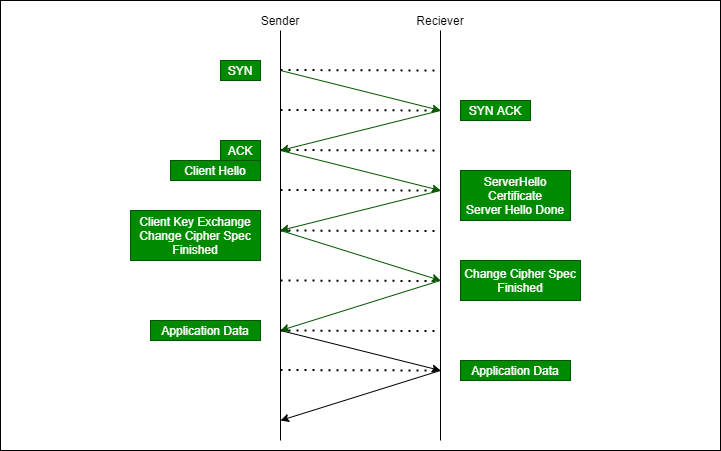
\includegraphics[scale=0.7]{tlsdiagram.png}
% \end{figure}




\section{Cipher Suites}

A cipher suite (for TLS1.2) looks like
\begin{center}
        \verb|TLS_ECDHE_ECDSA_WITH_AES_128_GCM_SHA256|    
\end{center}
It contains:
\begin{enumerate}
    \item Protocol: Transport Layer Security (TLS).
    \item Secret Key Exchange: Elliptic Curve Diffie Hellman Ephemeral (ECDHE).
    \item Public Key Authentication Method: Elliptic Curve Digital Signature Algorithm (ECDSA).
    \item AEAD Cipher: Advanced Encyrption Standard (AES) with key size 128bits with operations of GCM.
    \item PRF Hash algorithm: SHA256.
\end{enumerate}
So we can read it as 
\begin{center}
    Use Ephemeral Elliptic-Curve Diffie-Hellman (ECDHE) to establish a shared secret, authenticate the server using ECDSA signatures, encrypt all traffic using AES-128 in GCM mode, and use SHA-256 during the TLS 1.2 key-derivation and handshake process.
\end{center}

A cipher suite (for TLS1.3) looks like
\begin{center}
    \verb|TLS_AES_256_GCM_SHA384|
\end{center}
It contains:
\begin{enumerate}
    \item Protocol: Transport Layer Security (TLS).
    \item Secret Key Exchange: Elliptic Curve Diffie Hellman Ephemeral (ECDHE).
    \item Public Key Authentication Method: Elliptic Curve Digital Signature Algorithm (ECDSA).
    \item AEAD Cipher: Advanced Encyrption Standard (AES) with key size 128bits with operations of GCM.
    \item PRF Hash algorithm: SHA256.
\end{enumerate}

% \chapter{Advanced Encryption Standard (AES)}
% Advanced Encryption Standard (AES) is a variant of Rijndael block cipher that is established by NIST and adopted by US government. FIPS 197 is the United States federal computer security standard that defines the AES. AES is a block cipher (encryption and decryption on a $4x4$ block of bytes)



% \section{On OpenSSL}

% \begin{enumerate}
%     \item First create a plain text message in a file.
%     \begin{lstlisting}[style=darkbash, language=bash]
%     echo "This is a secret message!" > plaintext.txt
%     \end{lstlisting}
%     \item Here are the list of encodings we can use to encrypt
%     \begin{lstlisting}[style=darkbash, language=bash]
%     openssl enc -list
%     \end{lstlisting}
%     We chose \texttt{aes-256-cbc} for now
%     \begin{lstlisting}[style=darkbash, language=bash]
%     openssl enc -aes-256-cbc -salt -in plaintext.txt -out encrypted.bin
%     \end{lstlisting}
%     You will be prompted for a password.
%     \item We can then decrypt
%     \begin{lstlisting}[style=darkbash, language=bash]
%     openssl enc -d -aes-256-cbc -in encrypted.bin -out decrypted.txt
%     \end{lstlisting} 
%     \item
%     A modern version of encryption-decryption would be 
%     \begin{lstlisting}[style=darkbash, language=bash]
%     openssl enc -aes-256-cbc -pbkdf2 -iter 10000\
%     -in plaintext.txt \
%     -out encrypted.bin
%     \end{lstlisting} 
%     and 
%     \begin{lstlisting}[style=darkbash, language=bash]
%     openssl -d enc -aes-256-cbc -pbkdf2 -iter 10000\
%     -in encrypted.bin \
%     -out decrypted.txt
%     \end{lstlisting} 
% \end{enumerate}


\chapter{Cryptanalysis and Attacks}


% ref: Pro Cryptography and Cryptanalysis with C23
\section{Security analysis}
This section presents a security analysis using techniques for finding the weakness or security breaches in the cryptosystem. The following methods, techniques, and analysis should be considered when designing a chaotic system or conducting a cryptanalytic attack.

\begin{enumerate}
    \item \emph{Keyspace analysis}: The number of trials for finding the
 ecryption key and is made by trying all the possible keys from the keyspace of the encryption system. Note that the keyspace grows exponentially and simultaneously with the increment of the key's size.
    \item \emph{Secret key sensitivity analysis}: It is important to a good image encryption system. If just a single bit is modified in the secret key, then the output image should be a completely different image (regarding encryption or decryption).
    \item \emph{Statistical analysis} proves the relationship between the original image and the encrypted image.
    \item \emph{Correlation coefficient analysis} is an important graphical tool that needs to be studied in the histogram, namely, the distribution of the values generated by a trajectory of a dynamic system. Among the histogram analysis, the correlation between the pixels of a plain image and the encrypted image is another important technique, as it is made between two pixels distributed vertically, horizontally, and diagonally.
    \item \emph{Information entropy analysis} is based on entropy tests of the robustness of the encryption algorithm. The comparison between the entropy of the plain image and the encrypted image is very important, which shows that the entropy of the encrypted images is approximately 8-bit depth. This is useful in proving the encryption technique against the entropy attack.
    \item \emph{Differential analysis} determines the sensitivity of the cryptosystem regarding any slight change in the algorithm. The sensitivity can be computed based on two criteria: NPCR (Number of Pixels Change Rate) and UACI (Unified Average Changing Intensity). When these tests are made, the high values show the small changes in the plain image that produced significant modifications in the encrypted image.
\end{enumerate}

\begin{table}[ht]
\centering
\caption{Chaotic Map (Systems) for Image Encryption}
\label{tab:chaotic_maps}
\begin{tabular}{lccccc}
\toprule
\multirow{2}{*}{\textbf{Chaotic Map (System)}} &
\multicolumn{3}{c}{\textbf{Metrics}} &
\multicolumn{2}{c}{\textbf{Key}} \\
\cmidrule(lr){2-4}
\cmidrule(lr){5-6}
 & \textbf{Entropy} & \textbf{NPCR} & \textbf{UACI} &
\textbf{Space} & \textbf{Sensitivity} \\
\midrule
Lorenz Baker      & 7.9973 & --        & --        & $2^{128}$ & High   \\
Lorenz            & --     & --        & --        & Large     & Medium \\
Henon Map         & 7.9904 & 0.0015\%  & 0.0005\%  & $2^{128}$ & High   \\
Logistic Map      & 7.9996 & 99.6231\% & 33.4070\% & $10^{45}$ & High   \\
Trigonometry Maps & --     & 0.25\%    & 0.19\%    & $2^{302}$ & --     \\
Arnold Cat Map    & 7.9981 & 99.62\%   & 33.19\%   & $2^{148}$ & High   \\
Chebyshev Map     & 7.9902 & 99.609\%  & 33.464\%  & $2^{167}$ & High   \\
Circle Map        & 7.9902 & 99.63\%   & 33\%      & $2^{256}$ & High   \\
Arnold Map        & --     & 0.0015\%  & 0.004\%   & --        & --     \\
\bottomrule
\end{tabular}
\end{table}




% \chapter{Post-Quantum  Cryptography}

% \section{In OpenSSL}

% \subsection{Key Encapsulation Mechanism (KEM)}

% \begin{enumerate}
%     \item Verify that your installation supports native PQC algorithms:
%     \begin{lstlisting}[style=darkbash, language=bash]
%     openssl version
%     openssl list -kem-algorithms
%     openssl list -signature-algorithms
%     \end{lstlisting}
%     \item Key Encapsulation Mechanism (ML-KEM)
%     \begin{lstlisting}[style=darkbash, language=bash]
%     openssl genpkey -algorithm ml-kem-768 -out alice_private.pem
%     openssl pkey -in alice_private.pem -pubout -out alice_public.pem
%     \end{lstlisting}
%     \item Encapsulate a secret using the public key (Bob's side)
%     \begin{lstlisting}[style=darkbash, language=bash]
%     openssl pkeyutl -encap -pubin -inkey alice_public.pem -secret shared_bob.dat -out ciphertext.dat
%     \end{lstlisting}
%     \item Decapsulate the ciphertext using the private key (Alice's side):
%     \begin{lstlisting}[style=darkbash, language=bash]
%     openssl pkeyutl -decap -inkey alice_private.pem \
%     -in ciphertext.dat \ 
%     -out shared_alice.dat
%     \end{lstlisting}
%     \item Verify the shared secrets match
%     \begin{lstlisting}[style=darkbash, language=bash]
%     xxd shared_bob.dat
%     xxd shared_alice.dat
%     \end{lstlisting} 
% \end{enumerate}






\chapter{Appendices}


\section{Tools and Libraries}
We can use the following tools
\begin{enumerate}
    \item \verb|curl|.
    \item \verb|openssl|.
    \item \verb|openssh|.
\end{enumerate}


\section{Important Organizations}
Here are important organizations with their links that we need to follow as a cybersecurity expert:
\begin{enumerate}
    \item \href{https://csrc.nist.gov/}{NIST}.
\end{enumerate}




\section{Jargon}
\begin{longtable}{|lp{10cm}|} \hline 
    Nonce & number use once. \\ \hline 
    Protocol & A set of rules and format for exchanging of information \\ \hline 
    Ephemeral & New key pair generated in each TLS session \\ \hline 
    Fuzzing (or fuzz testing) & An automated software testing method that sends random, bad, or unexpected data into a program. It watches the program to see if it crashes, leaks memory, or breaks \\ \hline 
    \caption{Common Terminology} 
\end{longtable}


\section{Adages}

\emph{Kerckhoff's principle}: The security of the symmetric encryption depends on the secrecy of the key, not the secrecy of the algorithm.

\emph{Shannon's Maxim}: The enemy knows the system.


\emph{Principle of Least Privilege}: Give every user, process, or program only the minimum permissions necessary.


\section{Abbreviations}

\begin{longtable}{||lp{11cm}||} \hline 
    .PEM & Privacy-Enhanced Mail file format \\ \hline 
    3DES & Triple Data Encryption Standard \\ \hline 
    AAD & Additional Authenticated Data \\ \hline 
    AE & Authenticated Encryption \\ \hline 
    AEAD & Authenticated Encryption with Associated \newline Data algorithms \\ \hline 
    AES & Advanced Encyrption Standard \\ \hline 
    AKS test & Agrawal-Kayal-Saxena primality test \\ \hline 
    AMD & Advanced Micro Devices \\ \hline 
    ANSI & American National Standards Institute \\ \hline 
    ASCII & American Standard Code for Information Interchange \\ \hline  
    ATM & Automatic Teller Machine \\ \hline 
    BBS & Blum-Blum-Shub \\ \hline 
    BDH & Bilinear Diffie-Hellman \\ \hline 
    BPP & Bounded-error Probabilistic Polynomial time \\ \hline 
    BSGS & Baby-Step Giant-Step \\ \hline 
    CA & Certificate Authority \\ \hline 
    CAPTCHA & Completely Automated ProgramtoTell Computersand Humans Apart \\ \hline 
    CBC & Cipher Block Chaining \\ \hline 
    CCA & Chosen Ciphertext Attack \\ \hline 
    CCB & Counter with CBC-MAC \\ \hline 
    CCRA & Computational Composite Residuosity Assumption \\ \hline 
    CDH & Computational Diffie-Hellman \\ \hline 
    CFB & Cipher Feedback \\ \hline 
    CMA & Chosen Message Attack \\ \hline 
    CMAC & Cipher-based Message Authentication Code \\ \hline 
    CPA & Chosen Plaintext Attack \\ \hline 
    CPP & Cyclotomy Primality Proving \\ \hline 
    CPU & Central Processing Unit \\ \hline 
    CRC & Cyclic Redundancy Check \\ \hline 
    CRL & Certificate Revocation List \\ \hline 
    CRT & Chinese Remainder Theorem \\ \hline 
    CTR & CounTeR \\ \hline 
    DCRA & Decisional Composite Residuosity Assumption \\ \hline 
    DDH & Decisional Diffie-Hellman \\ \hline 
    DE & full Disk Encryption \\ \hline 
    DEM & Data Encapsulation Mechanism \\ \hline 
    DES & Data Encryption Standard \\ \hline
    DH & Diffie Hellman algorithm \\ \hline 
    DL & Discrete Logarithm \\ \hline 
    DLP & Discrete Logarithm Problem \\ \hline 
    DNS & Domain Name Resolution \\ \hline
    DRBG & Deterministic Random Bit Generator \\ \hline 
    DSA & Digital Signature Algorithm \\ \hline 
    EAP & Extensible Authentication Protocol \\ \hline 
    EC & Elliptic Curve \\ \hline 
    ECB & Electronic Code Book \\ \hline 
    ECC & Elliptic Curve Cryptography \\ \hline 
    ECDH & Elliptic Curve Diffie-Hellman algorithm \\ \hline 
    ECDHE & Elliptic Curve Diffie-Hellman Ephemeral algorithm \\ \hline 
    ECDLP & Elliptic Curve DLP \\ \hline 
    ECDSA & Elliptic Curve Digital Signature Algorithm \\ \hline 
    ECIES & Elliptic Curve Integrated Encryption Scheme \\ \hline 
    ECM & Elliptic Curve Method \\ \hline 
    ECPP & Elliptic Curve Primality Proving \\ \hline 
    ECRYPT & European Network of Excellence in Cryptology \\ \hline 
    EME-OAEP & Encoding Method for Encryption-OAEP \\ \hline 
    EMSA-PSS & Encoding Method for Signature with Appendix-PSS \\ \hline 
    EPFL & \'Ecole Polytechnique F\'ed\'erale de Lausanne \\ \hline 
    ERH & Extended Riemann Hypothesis \\ \hline 
    FDH & Full Domain Hash \\ \hline 
    FEDER & Fonds Europ\'een de D\'eveloppement R\'egional \\ \hline 
    FIPS & Federal Information Processing Standards \\ \hline 
    FNISA & French Network and Information Security Agency \\ \hline 
    FNMT & F\'abrica Nacional de Moneda y Timbre \\ \hline 
    FR & Frey-R\"uck \\ \hline 
    FTP & File Transfer Protocol \\ \hline 
    gcd & greatest common divisor \\ \hline 
    GCHQ & Government Communications Headquarters \\ \hline 
    GCM & Glois/Counter Mode of operation \\ \hline  
    GCTR & Galois Counter \\ \hline 
    GGH & Goldreich, Goldwasser, and Halevi  \\ \hline 
    GGNFS & GPL'd implementation of the General Number Field Sieve \\ \hline 
    GHASH & Galois HASH  \\ \hline 
    GMAC & Galois Message Authentication Code \\ \hline 
    GMP & GNU Multiple-Precision Arithmetic Library \\ \hline 
    GNFS & General Number Field Sieve \\ \hline 
    GNU & GNU's not Unix \\ \hline 
    GPL & General Public License \\ \hline 
    GSM & Global System for Mobile Communications \\ \hline 
    HMAC & keyed-Hash Message Authentication Code \\ \hline     
    HSM & Hardware Security Module \\ \hline 
    HTTP &  HyperText Transfer Protocol \\ \hline 
    IBC & Identity-Based Cryptography \\ \hline 
    IBE & Identity-Based Encryption \\ \hline 
    IBM & International Business Machines \\ \hline 
    IBS & Identity-Based Signatures \\ \hline 
    IC & Index of Coincidence \\ \hline 
    ICB & Initial Counter Block \\ \hline 
    IDEA & International Data Encryption Algorithm \\ \hline 
    IEC & International Electrotechnical Commission \\ \hline 
    IETF &  Internet Engineering Task Force \\ \hline 
    IFP & Integer Factorization Problem \\ \hline 
    IMAP & Internet Message Access Protocol \\ \hline 
    IND-CCA & Indistinguishable under CCA \\ \hline 
    IND-CCA1 & Indistinguishable under non-adaptive CCA \\ \hline 
    IND-CCA2 & Indistinguishable under adaptive CCA \\ \hline 
    IND-CPA & Indistinguishable under CPA \\ \hline 
    IND-EAV & Indistinguishable to Eavesdroppers \\ \hline 
    INT-CTXT & Ciphertext Integrity \\ \hline 
    INT-PTXT & Plaintext Integrity \\ \hline 
    IP & Internet Protocol \\ \hline 
    IPSec & Internet Protocol Security \\ \hline 
    ISO & International Organization for Standardization \\ \hline 
    IV & Initialization Vector \\ \hline 
    KCV & Ket Check Value \\ \hline 
    KDF & Key Derivation Function \\ \hline 
    KEM & Key Encapsulation Mechanism \\ \hline 
    KPI & Key Performance Indicators \\ \hline 
    KRI & Key Risk Indicators \\ \hline 
    lcm & least common multiple \\ \hline 
    LLL algorithm & Lenstra-Lenstra-Lov\'asz algorithm \\ \hline 
    LSB & Least Significant Bit \\ \hline 
    LWE problem & Learning With Error problem \\ \hline  
    MAC & Message Authentication Code \\ \hline 
    MAC address & Medium Access Control address \\ \hline 
    MitM attack & Man in the Middle attack \\ \hline 
    MD & Message Digest \\ \hline 
    MD5 & Message Digest 5 \\ \hline 
    MGF & Mask Generating Function \\ \hline 
    MIME & Multipurpose Internet Mail Extensions \\ \hline 
    MIRACL & Multiprecision Integer and Rational Arithmetic \newline  C/C++ Library \\ \hline 
    MIT & Massachusetts Institute of Technology \\ \hline 
    MOV & Menezes-Okamoto-Vanstone \\ \hline 
    MPQS & Multiple-Polynomial Quadratic Sieve \\ \hline 
    MSB & Most Significant Bit \\ \hline 
    NBS & National Bureau of Standards \\ \hline 
    NFS & Number Field Sieve \\ \hline 
    NIST & National Institute of Standards and Technology \\ \hline 
    NTRU & $N$-th degree Truncated polynomial Ring Units \\ \hline 
    NTRU & Number Theorists R Us \\ \hline 
    NM & Non-Malleable \\ \hline 
    NP & Non-deterministic Polynomial time \\ \hline 
    NSA & National Security Agency \\ \hline 
    OAEP & Optimal Asymmetric Encryption Padding \\ \hline
    OFB & Output Feedback \\ \hline 
    OMAC & One-key MAC \\ \hline
    OSI model & Open Systems Interconnection model \\ \hline
    OTP & One-Time Pad \\ \hline  
    OW-CCA & One-Way secure against CCA \\ \hline 
    OW-CPA & One-Way secure against CPA \\ \hline 
    P & Polynomial time \\ \hline 
    PDU & Protocol Data Units \\ \hline 
    PGP & Pretty Good Privacy \\ \hline 
    PII & Personally Identifiable Information \\ \hline
    PIN & Personal Identification Number \\ \hline 
    PKC & Public Key Cryptography  \\ \hline 
    PKCS & Public Key Cryptography Standards \\ \hline 
    PKG & Private-Key Generator \\ \hline 
    PKI & Public Key Infrastructure \\ \hline 
    PNT & Prime Number Theorem \\ \hline 
    POC & Proof Of Concept \\ \hline 
    POP3 & Post Office Protocol version 3 \\ \hline 
    POTP & Pseudo-Random One-Time Pad \\ \hline 
    PPT & Probabilistic Polynomial Time \\ \hline 
    PQC & Post-Quantum Cryptography \\ \hline 
    PRF & PseudoRandom Function \\ \hline 
    PRG & Pseudo-Random Generator \\ \hline 
    PRNG & Pseudo-Random Number Generator \\ \hline 
    PSS & Probabilistic Signature Scheme \\ \hline 
    PSW & Pomerance-Selfridge-Wagstaff \\ \hline 
    QR & Quadratic Residuosity \\ \hline 
    QS & Quadratic Sieve \\ \hline 
    RC4 & Rivest Cipher 4 \\ \hline 
    RFC & Request For Comments \\ \hline 
    RKA & Related-Key Attack \\ \hline 
    RP & Randomized Polynomial time \\ \hline 
    RREF & Reduced Row Echelon Form \\ \hline 
    RSA & Rivest, Shamir, Adleman algorithm \\ \hline 
    RSAES-OAEP & RSA Encryption Scheme-OAEP \\ \hline 
    RSASSA-PSS & RSA Signature Scheme with Appendix-PSS \\ \hline 
    SAEP & Simple OAEP \\ \hline 
    SEA & Schoof-Elkies-Atkin \\ \hline 
    SEC & Standards for Efficient Cryptography \\ \hline 
    SECG & Standards for Efficient Cryptography Group \\ \hline 
    SHA & Secure Hash Algorithm \\ \hline 
    SHS & Secure Hash Standard \\ \hline 
    SIQS & Self-Initializing Quadratic Sieve \\ \hline 
    SME & Subject Matter Expert \\ \hline 
    S/MIME & Secure MIME \\ \hline 
    SMTP & Simple Mail Transfer Protocol \\ \hline 
    SRTP & Secure Real-time Transport Protocol \\ \hline 
    SS-2-IBS & Standard Signatures to Identity-Based Signatures \\ \hline 
    SSH & Secure SHell \\ \hline 
    SSL & Secure Sockets Layer \\ \hline 
    SUF-CMA & Strongly Unforgeable under CMA \\ \hline 
    SVP & Shortest Vector Problem \\ \hline 
    TCP & Transmission Control Protocol \\ \hline 
    TKIP & Temporal Key Integrity Protocol \\ \hline 
    TLS & Transport Layer Security \\ \hline 
    UF-CMA & Unforgeable under CMA \\ \hline 
    UMAC & Universal MAC \\ \hline 
    URL & Uniform Resource Locator \\ \hline 
    VPN & Virtual Private Network \\ \hline 
    WEP & Wired Equivalent Privacy \\ \hline 
    WPA & Wi-Fi Protected Access \\ \hline 
    WPA2 & Wi-Fi Protected Access II \\ \hline 
    WPA3 & Wi-Fi Protected Access III \\ \hline 
    XCBC & eXtended CBC \\ \hline 
    XOR & Exclusive OR \\ \hline 
    XSL & eXtended Sparse Linearization \\ \hline 
    ZPP & Zero-error Probabilistic Polynomial time \\ \hline 
    \caption{Abbreviations}
\end{longtable}


\section{Hacking techniques}

\begin{longtable}{|lp{10cm}|} \hline 
    Phishing & A broad form of social engineering where attackers use spoofed emails or messages to emotionally manipulate victims into providing sensitive data. \\ \hline 
    Spoofing & A deceptive tactic where a cybercriminal, scammer, or malicious entity disguises their identity, device, or communication as a trusted source \\ \hline 
    Man-in-the-Middle (MitM) & An attack where the perpetrator secretly intercepts and alters communications between two parties. \\ \hline 
    Denial of Service (DoS) &  Flooding a network or server with traffic, sometimes using spoofed IP addresses to conceal the attack's origin \\ \hline 
    \caption{Jargon}
\end{longtable}


\section{Comparisons}

\begin{longtable}{||c|c||} \hline 
    Classical Diffie-Hellman & EC Diffie-Hellman \\
    On modular arithmetic & On elliptic curves \\ 
    Bigger key size & Smaller key size \\ \hline \hline 
\end{longtable}












% \chapter{References}

%-- Computation Engineering by Ganesh Gopalakrishnan

\cite{adamson2012set}

% \nocite{*}



\bibliography{references}
\bibliographystyle{amsalpha}

\printindex




\end{document}